\documentclass[11pt]{article}
\usepackage[margin=1in]{geometry}
\usepackage{volfit_preamble}
\graphicspath{{figures/}}

\title{\textbf{Event Time Dilation and the Variance Clock}\\[2pt]
\large Two clocks, day-weighted events, and a price-preserving vol drop\\[2pt]
\normalsize Vol-Fitter Technical Notes, No.~11}
\author{Vol-Fitter}
\date{\today}

\begin{document}
\maketitle
% Auto-generated by gen_event.py — do not edit.
\newcommand{\evtextra}{4}
\newcommand{\evtte}{0.25}
\newcommand{\evttauprobe}{0.3110}
\newcommand{\evtdropbp}{36}
\newcommand{\evtdays}{365}


\begin{abstract}
Variance does not accrue uniformly in calendar time: a scheduled event ---
earnings, an FOMC print, a court ruling --- packs the variance of several normal
days onto one. This note documents the Vol-Fitter's \emph{variance clock}, which
makes that explicit by carrying two times: calendar time $t$, and a dilated
variance time $\tau$ in which an event day counts as several. Each event adds a
number of \emph{extra equivalent days}; the surface is fitted and quoted in
weighted years $\tau=\tau_{\text{days}}/365$. The key invariant is
price-preservation: total variance $w(k)$ is fixed by the observed option price
and is clock-independent, so the working implied volatility $\sqrt{w/\tau}$
\emph{drops} when an event is inserted before the expiry --- exactly the
overnight-vol-crush traders expect. An optional normalization rescales all days so
the one-year variance budget is unchanged, making events \emph{redistribute}
variance within the year rather than add it. The calendar can be typed in or
\emph{auto-calibrated}: a solver places events so the event-time forward
variance is as flat as possible, inferring the calendar from the term
structure's kinks, after which it is editable. With no events the variance clock
collapses to calendar time and every downstream fit is byte-identical to the
plain pipeline. A worked example shows a $4$-extra-day earnings event lifting
short-dated implied vol and decaying away, with a working-vol drop of
\evtdropbp\ vol bps at a fixed expiry just past the event.
\end{abstract}

\tableofcontents
\newpage

%======================================================================
\section{Why two clocks}
\label{sec:why}

A diffusion model assumes variance accrues at a steady rate: total variance
$w=\sigma^2 t$ is linear in calendar time. Real markets violate this around
scheduled events, where a single day carries the variance of many. Forcing such a
surface onto a single calendar clock produces the familiar pathology --- a
short-dated implied vol that looks ``too high'' and a term structure with a kink
that a smooth model cannot represent without distorting the smile.

\begin{heuristic}
Separate the \emph{calendar} (how many days until expiry) from the \emph{variance
budget} (how much variance those days carry). An earnings day is one calendar day
but, say, five days' worth of variance. If we measure time in \emph{variance days},
the diffusion looks steady again --- and the ``too high'' short-dated implied vol
is just the same total variance divided by a smaller calendar time. The event
clock is the change of variable that restores $w=\sigma^2\tau$ with a constant
$\sigma$.
\end{heuristic}

\begin{invariant}
\begin{enumerate}[leftmargin=1.6em]
\item \textbf{Price preservation.} The clock never touches $w(k)$; it changes
only the volatility read-off $\sqrt{w/\tau}$. Adding an event cannot change an
option price, hence cannot introduce arbitrage.
\item With an empty calendar, $\tau=t$ exactly and the entire downstream
pipeline is byte-identical.
\item Every consumer --- every fit, the LV surface, the term structure, the
table --- reads the \emph{same} $\tau$; there is one variance clock per node,
not one per view.
\item Editing the calendar refits only the affected ticker (per-ticker events
version).
\end{enumerate}
\end{invariant}

%======================================================================
\section{The variance clock}
\label{sec:clock}

\subsection{Day-weighted variance time}

Each event carries a number $N_e$ of \emph{extra} equivalent days (an earnings day
with $N_e=4$ counts as $5$ normal days of variance). The variance time to a
calendar maturity $t$ is
\begin{equation}
\boxed{\;\tau_{\text{days}}(t)=t\cdot 365+\!\!\sum_{t_e\le t}\!N_e,
\qquad \tau(t)=\frac{\tau_{\text{days}}(t)}{365},\;}
\label{eq:clock}
\end{equation}
counting only events at or before $t$. \Cref{fig:clock} plots $\tau(t)$: it tracks
the calendar line until the event, jumps by $N_e/365$ there, and runs parallel
afterward. The fits and quotes live on $\tau$; with no events, $\tau(t)=t$ exactly.
The clock \eqref{eq:clock}, with the optional $1$Y-budget normalization, is direct
(matches production to $10^{-12}$):

\begin{lstlisting}[caption={The event variance clock $\tau(t)$ \eqref{eq:clock}
(distilled from \texttt{calib/weighted\_time.py::weighted\_variance\_years}).},
label={lst:clock}]
def weighted_variance_years(t_cal, events, normalize=False, dpy=365.0):
    if t_cal <= 0: return t_cal          # events: (t_e, N_e) pairs, N_e = extra days
    tau_days = t_cal*dpy + sum(N for te, N in events if te <= t_cal and N > 0)
    if normalize:                        # rescale so a 1Y budget stays dpy days
        e1 = sum(N for te, N in events if te <= 1.0 and N > 0)
        tau_days *= dpy/(dpy + e1)
    return tau_days/dpy                  # tau(t); equals t_cal with no events
\end{lstlisting}

\begin{figure}[H]
\centering
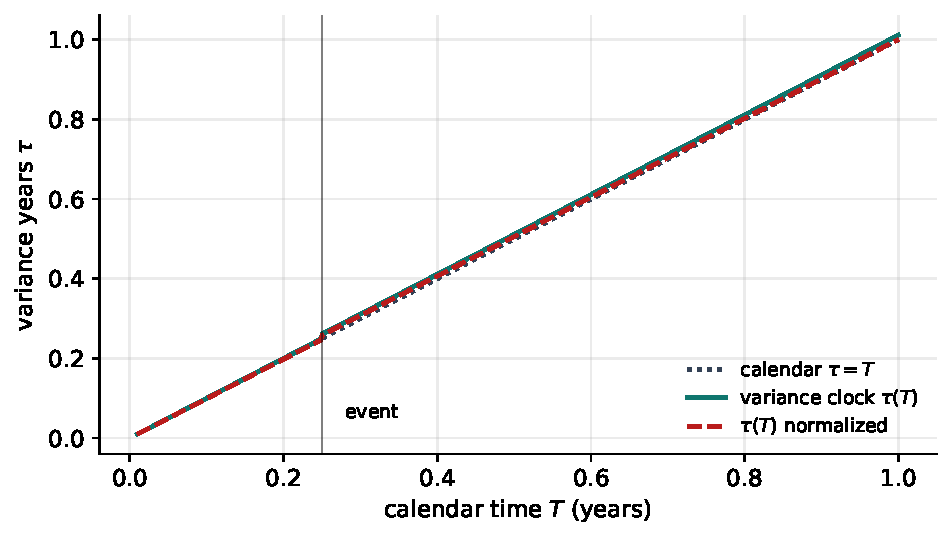
\includegraphics[width=0.74\textwidth]{fig_event_clock.pdf}
\caption{Variance time $\tau(t)$ for an event at $t_e=\evtte$ worth $\evtextra$
extra days: it jumps at the event and runs parallel to calendar time thereafter.
The normalized clock (dashed) rescales so the one-year budget is unchanged.}
\label{fig:clock}
\end{figure}

\subsection{Price preservation}

The crucial invariant is that the \emph{total variance} $w(k)$ is fixed by the
observed option price --- it is the Black total variance that reprices the quote,
and that is clock-independent. The variance clock only changes how we
\emph{report} it as a volatility:
\begin{equation}
\sigma_{\text{work}}(k)=\sqrt{\frac{w(k)}{\tau}}.
\label{eq:workvol}
\end{equation}
Inserting an event before the expiry raises $\tau$ at fixed $w$, so the working
implied vol \emph{drops}. This is the vol crush: the price is unchanged, but the
\emph{diffusive} volatility implied by it is lower once the event's variance is
accounted for separately. \Cref{fig:term} shows the term-structure consequence:
with the event, short-dated calendar implied vol is lifted (the event's variance
compressed into few calendar days) and decays as the event becomes a smaller
fraction of the maturity; without it, the term structure is flat.

\begin{figure}[H]
\centering
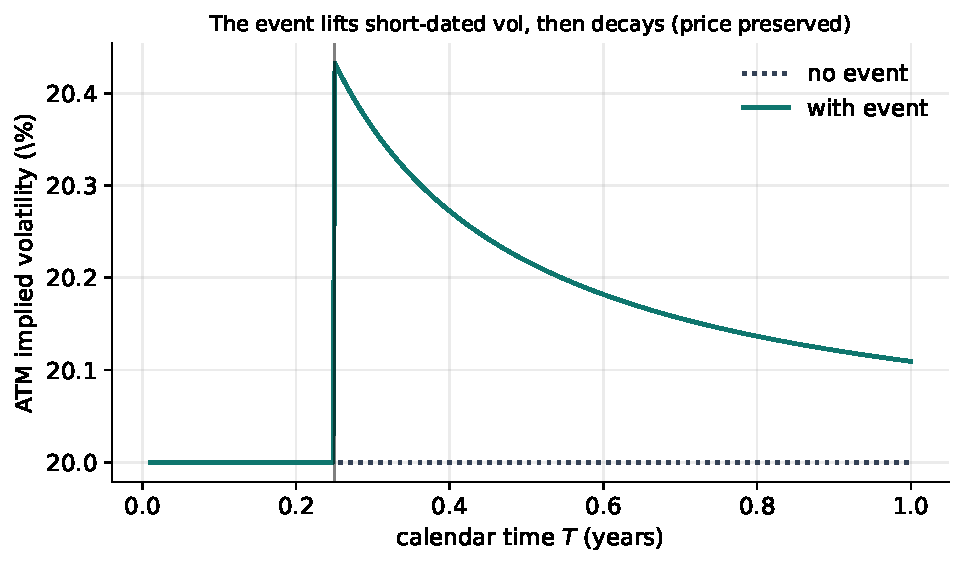
\includegraphics[width=0.74\textwidth]{fig_event_term.pdf}
\caption{ATM implied-vol term structure with and without the event. The event
lifts short-dated vol and decays away; the option \emph{prices} are preserved,
only the implied-vol reading changes.}
\label{fig:term}
\end{figure}

\subsection{Normalization}

By default the cumulative weight exceeds the calendar-day count ($\tau>t$). With
normalization on (an Options toggle), all days --- event days included --- are
rescaled by a single factor so the one-year weight budget stays $365$:
\begin{equation}
\tau_{\text{days}}(t)\ \longmapsto\ \tau_{\text{days}}(t)\cdot\frac{365}{365+\sum_{t_e\le1}N_e}.
\label{eq:normalize}
\end{equation}
Then the one-year variance time --- and the one-year implied vol --- are identical
to a no-event year: events only \emph{redistribute} variance within the year, they
do not add it. Which convention to use is a desk choice: un-normalized treats the
events as genuinely extra variance, normalized treats them as a known reallocation
of a fixed annual budget.

%======================================================================
\section{How it threads the pipeline}
\label{sec:thread}

The dual clock is prepared once per node by the clock of \cref{lst:clock}:
$\tau$ is stored as \texttt{prepared.tau} beside the calendar
\texttt{prepared.t}, and every fit (parametric and local-vol), the local-vol
grid, the term structure and the option table consume $\tau$ in place of
$t$.

\begin{remark}[One production clock, one legacy clock, one unit trap]
Two dilation clocks exist in the codebase and must not be conflated. The
production clock is \texttt{calib/weighted\_time.py} --- day-weighted, exactly
\eqref{eq:clock}, the one every fit consumes. The older
\texttt{calib/event\_time.py} (\texttt{EventClock}) survives only for
term-structure interpolation. And the unit trap: \texttt{weight} is
\emph{extra equivalent days}, never years --- confirmed both by the call site
(the pairs feed \eqref{eq:clock} directly) and by the auto-calibrator, which
constructs \texttt{EventSpec(weight=days)}. The \texttt{EventSpec} schema
docstring said \emph{years} until 2026-07-09 (now fixed to the day semantics
documented here); the legacy clock's comments remain the stale party.
\end{remark}

Total variance is
interpolated \emph{linearly in $\tau$} between quoted nodes --- flat forward
variance per weighted-time unit --- so the dense vol curve $\sqrt{w/\tau}$ stays
bounded near zero and sensible past the last expiry. The term-structure view uses
the shared calendar (not the per-node events) so the displayed curve is coherent
across expiries. Changing the event calendar bumps the per-ticker events version,
forcing a refit of only that name; with an empty calendar the whole pipeline is
byte-identical to calendar time.

Nor must the calendar be hand-entered. The Term workspace's
\emph{auto-calibrate} action infers it from the ATM term structure: placing
one candidate event before each expiry up to a chosen horizon
(\texttt{maxExpiry}), it solves for the non-negative extra days $N_e$ that
make the \emph{event-time} forward variance between consecutive expiries,
$(w_i-w_{i-1})/(\tau_i-\tau_{i-1})$, as flat and as monotone-increasing as
possible while keeping the events small and sparse (a bounded L-BFGS-B solve;
events under half a day are thresholded away, so the result is a short list).
The calendar-time forward variance $(w_i-w_{i-1})/(t_i-t_{i-1})$ is
event-\emph{invariant} --- prices fix $w$ --- so the objective works on the
dilated clock, the one events actually move: since an event can only
\emph{lengthen} an interval's weighted time, it pulls \emph{down} the
forward-variance spike an earnings-packed interval produces, toward its
neighbours. The calendar is thus read off exactly the kinks the clock was
built to explain, installed as the shared per-ticker calendar, and edited
like any hand-entered one (\nolinkurl{calib/event_autocalib.py},
\nolinkurl{api/event_autocalib.py}).

%======================================================================
\section{What is original here}
\label{sec:original}

Event time changes are not new in spirit (Bergomi and others dilate time around
events), but the implementation here has two clean properties worth singling out.
First, \emph{price preservation by construction}: the event clock never touches
$w(k)$, only the volatility read-off \eqref{eq:workvol}, so adding an event can
never change an option price --- it cannot introduce arbitrage. Second, the
\emph{day-weighted} parametrization \eqref{eq:clock} makes the event size a single
intuitive number (extra equivalent days) that a desk can quote and reason about,
with an optional budget normalization \eqref{eq:normalize} that cleanly separates
``extra variance'' from ``reallocated variance''. And the byte-identical fallback
when the calendar is empty means the feature is strictly additive. The payoff is
comparability: pre- and post-earnings surfaces line up across names and dates
because event-time vol is the signal --- calendar-time vol is the artifact.

%======================================================================
\section{Traceability}
\label{sec:traceability}

\begingroup
\small
\setlength{\tabcolsep}{3pt}
\begin{longtable}{@{}p{0.34\textwidth}p{0.10\textwidth}p{0.23\textwidth}p{0.29\textwidth}@{}}
\caption{Claims in this note and the code/tests that lock them.}\\
\toprule Claim & Object & Code anchor & Test anchor\\ \midrule
\endfirsthead
\toprule Claim & Object & Code anchor & Test anchor\\ \midrule
\endhead
No events: identity clock, byte-identical pipeline &
invariant~2 &
\nolinkurl{calib/weighted_time.py} &
\nolinkurl{test_weighted_time.py::test_no_events_is_identity}, \nolinkurl{::test_no_event_byte_identical}\\
Event adds day weights before its date only &
\eqref{eq:clock} &
\nolinkurl{calib/weighted_time.py} &
\nolinkurl{test_weighted_time.py::test_event_before_adds_day_weights}\\
Price preservation: IV drops by $\sqrt{t/\tau}$ &
\eqref{eq:workvol} &
\nolinkurl{api/service.py}, \nolinkurl{api/displayed.py} &
\nolinkurl{test_weighted_time.py::test_event_lowers_iv_by_sqrt_t_over_tau}, \nolinkurl{::test_localvol_iv_drops_with_event}\\
Normalization pins the one-year budget &
\eqref{eq:normalize} &
\nolinkurl{calib/weighted_time.py} &
\nolinkurl{test_weighted_time.py::test_normalization_pins_one_year}, \nolinkurl{::test_normalization_keeps_one_year_vol}\\
Surface mesh shares the smile's clock &
\cref{sec:thread} &
\nolinkurl{api/affine_views.py} &
\nolinkurl{test_surface_clock.py::test_surface_mesh_uses_variance_clock_like_the_smile}\\
Legacy clock confined to term interpolation &
remark &
\nolinkurl{calib/event_time.py} &
\nolinkurl{test_event_time.py::test_interpolation_lumps_event_variance}\\
Auto-calibrate flattens event-time forward variance; flat input stays
eventless &
\cref{sec:thread} &
\nolinkurl{calib/event_autocalib.py}, \nolinkurl{api/event_autocalib.py} &
\nolinkurl{test_event_autocalib.py::test_spike_is_flattened}, \nolinkurl{::test_flat_input_stays_eventless}\\
\bottomrule
\end{longtable}
\endgroup

\appendix
%======================================================================
\section{Hyperparameter atlas}
\label{app:atlas}

\begin{longtable}{p{0.26\textwidth}p{0.16\textwidth}p{0.50\textwidth}}
\caption{Event-clock hyperparameters.}\label{tab:atlas}\\
\toprule Knob & Default & Role\\ \midrule
\endfirsthead \toprule Knob & Default & Role\\ \midrule \endhead
\multicolumn{3}{l}{\emph{Surfaced (OptionsSettings)}}\\ \midrule
\texttt{events} & empty & List of \texttt{EventSpec}$(t_e,N_e,\text{label})$; $N_e$ = extra equivalent days.\\
\texttt{normalizeEvents} & off & Rescale all days to a fixed $365$ one-year budget \eqref{eq:normalize}.\\
\texttt{maxExpiry} & --- & Auto-calibrate horizon: one candidate event per
expiry at or before it (\cref{sec:thread}).\\
\midrule
\multicolumn{3}{l}{\emph{Hidden}}\\ \midrule
\texttt{DAYS\_PER\_YEAR} & $\evtdays$ & Calendar-to-variance day conversion.\\
\texttt{mono\_weight} & $1.0$ & Auto-calibrate: penalty on decreasing
event-time forward variance.\\
\texttt{sparse\_weight} / \texttt{ridge\_weight} & $10^{-3}$ / $10^{-4}$ &
Auto-calibrate: keep solved events small and sparse.\\
\texttt{min\_event\_days} & $0.5$ & Auto-calibrate sparsity threshold:
smaller solved events are dropped.\\
\bottomrule
\end{longtable}

\noindent\textbf{Performance.} The clock is a scalar sum per node, negligible.
With no events $\tau=t$ and the entire downstream pipeline is byte-identical, so
the feature adds zero cost when unused; changing the event calendar refits only the
affected ticker (per-ticker events version).

\begin{thebibliography}{9}
\bibitem{Bergomi2016} L.~Bergomi. \emph{Stochastic Volatility Modeling}. CRC Press,
2016.
\bibitem{Gatheral2006} J.~Gatheral. \emph{The Volatility Surface}. Wiley, 2006.
\end{thebibliography}

\end{document}
